\chapter{Signal Chain (End-to-End Processing)}
\label{ch:signal-chain}

\begin{nontechnical}
\textbf{The signal chain is like a postal system for data}---messages get packaged (encoded), addressed (modulated), mailed (transmitted), delivered (received), sorted (demodulated), and unpacked (decoded)!

\textbf{The complete journey:}
\begin{itemize}
\item \textbf{Sender:} You write a letter, put it in an envelope, add packing material for protection
\item \textbf{Post office:} Sorts, ships via airplane to destination
\item \textbf{Journey:} Package may get damaged, wet, or lost along the way
\item \textbf{Destination:} Arrives at receiver's local post office
\item \textbf{Receiver:} Opens package, removes packing, reads letter (hopefully intact!)
\end{itemize}

\textbf{Real example:} Sending an emoji via WiFi takes your 8-bit character through 11 processing stages in microseconds, surviving noise, interference, and multipath fading to arrive intact at your friend's phone.
\end{nontechnical}

\section{Overview}

The \textbf{signal chain} represents the complete end-to-end path that information takes from source to destination in a digital communication system. Understanding this chain is essential for analyzing system performance, diagnosing problems, and optimizing link budgets.

\begin{keyconcept}
Every stage in the signal chain introduces \textbf{impairments} (noise, distortion, loss) that degrade signal quality. The receiver's job is to undo these impairments and recover the original data with minimal errors. The signal chain provides a systematic framework for understanding where and how degradation occurs.
\end{keyconcept}

The signal chain consists of three major domains:
\begin{itemize}
\item \textbf{Transmitter:} Encodes, modulates, and radiates the signal
\item \textbf{Channel:} Attenuates, distorts, and adds noise to the signal
\item \textbf{Receiver:} Captures, demodulates, and decodes to recover data
\end{itemize}

\section{System Architecture}

\subsection{Complete Signal Chain Block Diagram}

The following diagram illustrates the complete end-to-end signal processing chain:

\begin{center}
\begin{tikzpicture}[
  block/.style={rectangle, draw, minimum width=2.2cm, minimum height=0.9cm, font=\sffamily\small, align=center},
  node distance=1.8cm,
  font=\small
]

% Transmitter chain
\node[font=\sffamily\bfseries] (txlabel) {Transmitter};
\node[block, below=0.4cm of txlabel] (data) {Data\\Source};
\node[block, below of=data] (fec) {FEC\\Encoder};
\node[block, below of=fec] (mod) {Modulator};
\node[block, below of=mod] (upconv) {Upconverter};
\node[block, below of=upconv] (txant) {TX\\Antenna};

% Channel
\node[block, below of=txant, minimum height=1.5cm, minimum width=2.2cm, fill=black!10!white] (channel) {Channel\\(Loss + Noise)};

% Receiver chain  
\node[block, below of=channel] (rxant) {RX\\Antenna};
\node[block, below of=rxant] (downconv) {Downconverter};
\node[block, below of=downconv] (sync) {Sync \&\\Equalize};
\node[block, below of=sync] (demod) {Demodulator};
\node[block, below of=demod] (decoder) {FEC\\Decoder};
\node[block, below of=decoder] (sink) {Data\\Sink};
\node[font=\sffamily\bfseries, below=0.4cm of sink] (rxlabel) {Receiver};

% Annotations
\node[right=0.3cm of data, font=\scriptsize, align=left] {Information bits\\$\{0,1\}$};
\node[right=0.3cm of fec, font=\scriptsize, align=left] {Coded bits\\(redundancy added)};
\node[right=0.3cm of mod, font=\scriptsize, align=left] {Complex symbols\\$I + jQ$};
\node[right=0.3cm of upconv, font=\scriptsize, align=left] {RF signal\\$f_c$ = GHz};
\node[right=0.3cm of channel, font=\scriptsize, align=left] {AWGN + Fading\\Link loss};
\node[right=0.3cm of downconv, font=\scriptsize, align=left] {Baseband\\$I + jQ$};
\node[right=0.3cm of demod, font=\scriptsize, align=left] {Soft bits\\(LLRs)};
\node[right=0.3cm of decoder, font=\scriptsize, align=left] {Decoded bits\\$\{0,1\}$};

% Arrows
\draw[->,thick] (data) -- (fec);
\draw[->,thick] (fec) -- (mod);
\draw[->,thick] (mod) -- (upconv);
\draw[->,thick] (upconv) -- (txant);
\draw[->,thick] (txant) -- (channel);
\draw[->,thick] (channel) -- (rxant);
\draw[->,thick] (rxant) -- (downconv);
\draw[->,thick] (downconv) -- (sync);
\draw[->,thick] (sync) -- (demod);
\draw[->,thick] (demod) -- (decoder);
\draw[->,thick] (decoder) -- (sink);

\end{tikzpicture}
\end{center}

\subsection{Transmitter Signal Flow}

\begin{center}
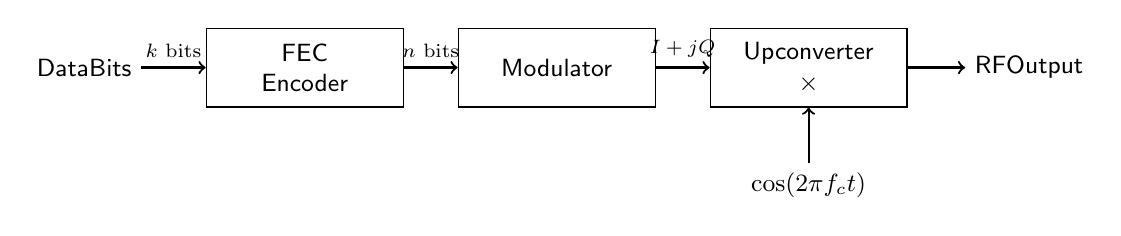
\begin{tikzpicture}[
  block/.style={rectangle, draw, minimum width=2.5cm, minimum height=1cm, font=\sffamily\small, align=center},
  node distance=3.2cm,
  font=\small
]
\node (input) {\sffamily Data\\Bits};
\node[block, right of=input, node distance=2.8cm] (fec) {FEC\\Encoder};
\node[block, right of=fec] (mod) {Modulator};
\node[block, right of=mod] (upconv) {Upconverter\\$\times$};
\node[right of=upconv, node distance=2.8cm] (output) {\sffamily RF\\Output};

\node[below of=upconv, node distance=1.5cm, font=\small] (lo) {$\cos(2\pi f_c t)$};

\draw[->,thick] (input) -- (fec) node[midway,above,font=\scriptsize] {$k$ bits};
\draw[->,thick] (fec) -- (mod) node[midway,above,font=\scriptsize] {$n$ bits};
\draw[->,thick] (mod) -- (upconv) node[midway,above,font=\scriptsize] {$I+jQ$};
\draw[->,thick] (lo) -- (upconv);
\draw[->,thick] (upconv) -- (output);
\end{tikzpicture}
\end{center}

\subsection{Receiver Signal Flow}

\begin{center}
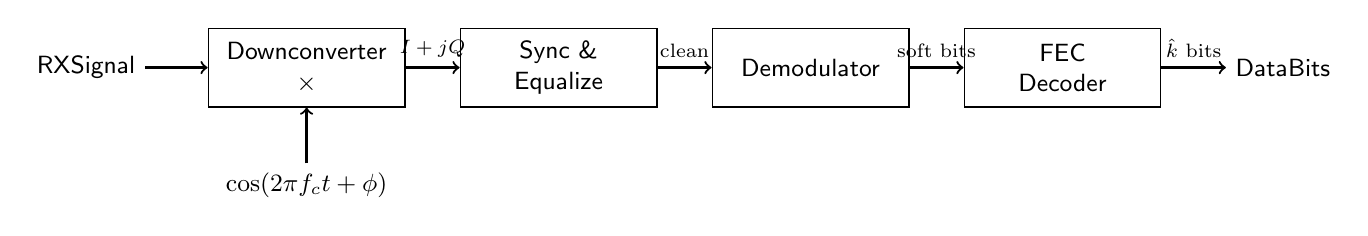
\begin{tikzpicture}[
  block/.style={rectangle, draw, minimum width=2.5cm, minimum height=1cm, font=\sffamily\small, align=center},
  node distance=3.2cm,
  font=\small
]
\node (input) {\sffamily RX\\Signal};
\node[block, right of=input, node distance=2.8cm] (downconv) {Downconverter\\$\times$};
\node[block, right of=downconv] (sync) {Sync \&\\Equalize};
\node[block, right of=sync] (demod) {Demodulator};
\node[block, right of=demod] (fec) {FEC\\Decoder};
\node[right of=fec, node distance=2.8cm] (output) {\sffamily Data\\Bits};

\node[below of=downconv, node distance=1.5cm, font=\small] (lo) {$\cos(2\pi f_c t + \phi)$};

\draw[->,thick] (input) -- (downconv);
\draw[->,thick] (lo) -- (downconv);
\draw[->,thick] (downconv) -- (sync) node[midway,above,font=\scriptsize] {$I+jQ$};
\draw[->,thick] (sync) -- (demod) node[midway,above,font=\scriptsize] {clean};
\draw[->,thick] (demod) -- (fec) node[midway,above,font=\scriptsize] {soft bits};
\draw[->,thick] (fec) -- (output) node[midway,above,font=\scriptsize] {$\hat{k}$ bits};
\end{tikzpicture}
\end{center}

\section{Mathematical Description}

\subsection{Data Rate Relationships}

The information bit rate $R_b$ relates to symbol rate $R_s$ through:
\begin{equation}
R_s = \frac{R_b}{m \cdot r_c}
\end{equation}
where:
\begin{itemize}
\item $R_b$ = information bit rate (bps)
\item $R_s$ = symbol rate (symbols/second)
\item $m = \log_2(M)$ = bits per symbol (e.g., $m=2$ for QPSK)
\item $r_c$ = code rate (e.g., $r_c = 1/2$ for rate-1/2 FEC)
\end{itemize}

\textbf{Example:} For $R_b = 1$ Mbps with QPSK ($m=2$) and rate-1/2 FEC ($r_c = 0.5$):
\begin{equation}
R_s = \frac{10^6}{2 \times 0.5} = 10^6\ \text{symbols/sec}
\end{equation}

\subsection{Signal Energy Relationships}

The energy per bit relates to symbol energy:
\begin{equation}
E_b = \frac{E_s}{m \cdot r_c}
\end{equation}
where:
\begin{itemize}
\item $E_b$ = energy per information bit (Joules)
\item $E_s$ = energy per symbol (Joules)
\item $m$ = bits per symbol
\item $r_c$ = code rate
\end{itemize}

Signal power relates to bit energy:
\begin{equation}
P_s = E_b \cdot R_b
\end{equation}
where:
\begin{itemize}
\item $P_s$ = average signal power (Watts)
\item $E_b$ = energy per bit (Joules)
\item $R_b$ = bit rate (bits/second)
\end{itemize}

\subsection{Channel Signal-to-Noise Ratio}

The channel SNR is defined as:
\begin{equation}
\mathrm{SNR} = \frac{P_s}{P_n} = \frac{P_s}{N_0 \cdot B}
\end{equation}
where:
\begin{itemize}
\item $P_s$ = signal power (Watts)
\item $P_n$ = noise power (Watts)
\item $N_0$ = noise power spectral density (W/Hz)
\item $B$ = signal bandwidth (Hz)
\end{itemize}

The relationship between SNR and $E_b/N_0$ is:
\begin{equation}
\frac{E_b}{N_0} = \mathrm{SNR} \cdot \frac{B}{R_b}
\end{equation}

\section{Transmitter Components}

\subsection{FEC Encoder}

\textbf{Purpose:} Add redundancy to enable error correction at the receiver.

\textbf{Input:} $k$ information bits\\
\textbf{Output:} $n$ coded bits ($n > k$)

The code rate is defined as:
\begin{equation}
r_c = \frac{k}{n}
\end{equation}
where:
\begin{itemize}
\item $k$ = number of information bits
\item $n$ = number of coded bits (including parity)
\item $r_c$ = code rate (e.g., 1/2, 2/3, 3/4)
\end{itemize}

\begin{calloutbox}{Common FEC Codes}
\begin{itemize}
\item \textbf{LDPC codes:} Excellent performance near Shannon limit
\item \textbf{Turbo codes:} Good performance, higher complexity
\item \textbf{Convolutional codes:} Lower complexity, continuous operation
\item \textbf{Reed-Solomon:} Burst error correction
\end{itemize}
\end{calloutbox}

\subsection{Modulator}

\textbf{Purpose:} Map coded bits to complex symbols in the constellation.

\textbf{Input:} $n$ coded bits\\
\textbf{Output:} $n/(m)$ complex symbols

The modulator groups $m = \log_2(M)$ bits per symbol:
\begin{equation}
N_s = \frac{n}{m}
\end{equation}
where:
\begin{itemize}
\item $N_s$ = number of symbols
\item $n$ = number of coded bits
\item $m = \log_2(M)$ = bits per symbol
\item $M$ = modulation order (e.g., $M=4$ for QPSK)
\end{itemize}

Each symbol is represented as:
\begin{equation}
s_i = I_i + jQ_i
\end{equation}
where $I_i$ and $Q_i$ are the in-phase and quadrature components.

\subsection{Upconverter}

\textbf{Purpose:} Shift baseband signal to RF carrier frequency.

The upconverted signal is:
\begin{equation}
s_{\mathrm{RF}}(t) = \mathrm{Re}\{s(t) \cdot e^{j2\pi f_c t}\} = I(t)\cos(2\pi f_c t) - Q(t)\sin(2\pi f_c t)
\end{equation}
where:
\begin{itemize}
\item $s(t) = I(t) + jQ(t)$ = complex baseband signal
\item $f_c$ = carrier frequency (Hz)
\item $s_{\mathrm{RF}}(t)$ = real-valued RF signal
\end{itemize}

\section{Channel Impairments}

\subsection{Link Loss}

The received power is attenuated by free-space path loss:
\begin{equation}
P_r = P_t + G_t + G_r - L_{\mathrm{path}}
\end{equation}
where (in dB):
\begin{itemize}
\item $P_r$ = received power (dBm)
\item $P_t$ = transmitted power (dBm)
\item $G_t$ = transmit antenna gain (dBi)
\item $G_r$ = receive antenna gain (dBi)
\item $L_{\mathrm{path}}$ = path loss (dB)
\end{itemize}

Free-space path loss is calculated as:
\begin{equation}
L_{\mathrm{FSPL}} = 20\log_{10}(d_{\mathrm{km}}) + 20\log_{10}(f_{\mathrm{MHz}}) + 32.45
\end{equation}

\begin{warningbox}
Path loss increases with \textbf{distance squared} and \textbf{frequency squared}. Doubling the distance adds 6 dB loss. Doubling the frequency adds 6 dB loss. These combine to make high-frequency long-range links extremely challenging.
\end{warningbox}

\subsection{Additive White Gaussian Noise (AWGN)}

Thermal noise is added to the signal:
\begin{equation}
r(t) = s(t) + n(t)
\end{equation}
where:
\begin{itemize}
\item $r(t)$ = received signal
\item $s(t)$ = transmitted signal (attenuated)
\item $n(t) \sim \mathcal{N}(0, \sigma^2)$ = AWGN
\end{itemize}

Noise power is:
\begin{equation}
P_n = N_0 \cdot B = kT_s B
\end{equation}
where:
\begin{itemize}
\item $k = 1.38 \times 10^{-23}$ J/K = Boltzmann constant
\item $T_s$ = system noise temperature (Kelvin)
\item $B$ = signal bandwidth (Hz)
\end{itemize}

\subsection{Multipath Fading}

Multiple signal copies arrive with different delays:
\begin{equation}
r(t) = \sum_{i=1}^{L} \alpha_i s(t - \tau_i) + n(t)
\end{equation}
where:
\begin{itemize}
\item $L$ = number of paths
\item $\alpha_i$ = attenuation of path $i$
\item $\tau_i$ = delay of path $i$
\end{itemize}

\section{Receiver Components}

\subsection{Downconverter}

\textbf{Purpose:} Shift RF signal back to baseband for digital processing.

The downconverted signal is:
\begin{equation}
r_b(t) = r_{\mathrm{RF}}(t) \cdot e^{-j2\pi f_c t}
\end{equation}
where:
\begin{itemize}
\item $r_b(t)$ = complex baseband signal
\item $r_{\mathrm{RF}}(t)$ = received RF signal
\item $f_c$ = local oscillator frequency (Hz)
\end{itemize}

After filtering, the baseband components are:
\begin{equation}
r_b(t) = I(t) + jQ(t)
\end{equation}

\subsection{Synchronization and Equalization}

\textbf{Synchronization} corrects timing, frequency, and phase offsets:
\begin{itemize}
\item \textbf{Timing synchronization:} Determine optimal sampling instants
\item \textbf{Carrier frequency offset:} Correct frequency mismatch $\Delta f$
\item \textbf{Phase offset:} Align carrier phase $\phi$
\end{itemize}

The timing error causes SNR degradation:
\begin{equation}
\mathrm{SNR}_{\mathrm{loss}} = 20\log_{10}\left(\mathrm{sinc}\left(\frac{\Delta t}{T_s}\right)\right)
\end{equation}
where $\Delta t$ is the timing error and $T_s$ is the symbol period.

\textbf{Equalization} compensates for channel distortion caused by multipath. The equalizer applies the inverse channel response:
\begin{equation}
H_{\mathrm{eq}}(f) \approx \frac{1}{H_{\mathrm{ch}}(f)}
\end{equation}

\subsection{Demodulator}

\textbf{Purpose:} Convert received symbols to bit estimates.

\textbf{Input:} Complex symbols $r_i = I_i + jQ_i$\\
\textbf{Output:} Soft bit estimates (log-likelihood ratios)

For hard decisions, the demodulator selects the nearest constellation point:
\begin{equation}
\hat{s}_i = \arg\min_{s \in \mathcal{S}} |r_i - s|
\end{equation}

For soft decisions (better for FEC decoding), compute log-likelihood ratios:
\begin{equation}
\mathrm{LLR}(b_k) = \log\frac{P(b_k = 0 | r)}{P(b_k = 1 | r)}
\end{equation}

\subsection{FEC Decoder}

\textbf{Purpose:} Detect and correct errors using redundancy.

\textbf{Input:} $n$ soft bits (LLRs)\\
\textbf{Output:} $k$ decoded information bits

The decoder uses iterative algorithms (e.g., belief propagation for LDPC) to converge on the most likely transmitted codeword. 

The coding gain is the SNR improvement:
\begin{equation}
G_c = \left(\frac{E_b}{N_0}\right)_{\mathrm{uncoded}} - \left(\frac{E_b}{N_0}\right)_{\mathrm{coded}}
\end{equation}
typically 5--10 dB for modern codes at BER $= 10^{-5}$.

\section{Performance Analysis}

\subsection{End-to-End Performance Metrics}

\begin{center}
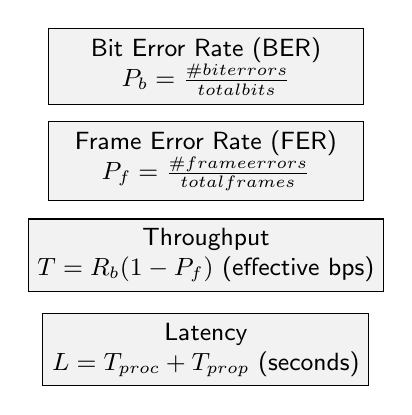
\begin{tikzpicture}[
  block/.style={rectangle, draw, minimum width=4cm, minimum height=0.8cm, font=\sffamily\small, align=center},
  node distance=1.2cm,
  font=\small
]
\node[block, fill=black!5!white] (ber) {Bit Error Rate (BER)\\$P_b = \frac{\text{\# bit errors}}{\text{total bits}}$};
\node[block, below of=ber, fill=black!5!white] (fer) {Frame Error Rate (FER)\\$P_f = \frac{\text{\# frame errors}}{\text{total frames}}$};
\node[block, below of=fer, fill=black!5!white] (throughput) {Throughput\\$T = R_b (1 - P_f)$ (effective bps)};
\node[block, below of=throughput, fill=black!5!white] (latency) {Latency\\$L = T_{\text{proc}} + T_{\text{prop}}$ (seconds)};
\end{tikzpicture}
\end{center}

\subsection{Processing Gain}

When spread spectrum techniques are used, processing gain improves the effective SNR:
\begin{equation}
G_p = \frac{R_{\mathrm{chip}}}{R_{\mathrm{symbol}}}
\end{equation}
where:
\begin{itemize}
\item $G_p$ = processing gain (ratio)
\item $R_{\mathrm{chip}}$ = chip rate (chips/second)
\item $R_{\mathrm{symbol}}$ = symbol rate (symbols/second)
\end{itemize}

In dB:
\begin{equation}
G_{p,\mathrm{dB}} = 10\log_{10}(G_p)
\end{equation}

The effective SNR at the demodulator is:
\begin{equation}
\mathrm{SNR}_{\mathrm{eff}} = \mathrm{SNR}_{\mathrm{channel}} + G_{p,\mathrm{dB}}
\end{equation}

\begin{calloutbox}{Example: Processing Gain Calculation}
\begin{itemize}
\item Symbol rate: $R_s = 3{,}200$ symbols/sec
\item Chip rate: $R_c = 32{,}000$ chips/sec
\item Spread factor: $G_p = 32{,}000 / 3{,}200 = 10$
\item Processing gain: $G_{p,\mathrm{dB}} = 10\log_{10}(10) = 10$ dB
\end{itemize}

If channel SNR = $-25$ dB, effective SNR = $-25 + 10 = -15$ dB.
\end{calloutbox}

\section{Worked Example: WiFi Link Budget}

\textbf{Scenario:} Calculate the link budget for an indoor WiFi system.

\subsection*{Given Parameters}

\begin{tabular}{@{}ll@{}}
TX power & $P_t = 20$ dBm (100 mW) \\
TX antenna gain & $G_t = 2$ dBi \\
Frequency & $f = 2.4$ GHz \\
Distance & $d = 10$ m \\
RX antenna gain & $G_r = 2$ dBi \\
System noise temp & $T_s = 290$ K (room temperature) \\
Bandwidth & $B = 20$ MHz \\
Modulation & QPSK ($m = 2$) \\
FEC code rate & $r_c = 1/2$ \\
Required BER & $10^{-5}$ \\
\end{tabular}

\subsection*{Step 1: Calculate Free-Space Path Loss}

\begin{equation}
L_{\mathrm{FSPL}} = 20\log_{10}(0.01) + 20\log_{10}(2400) + 32.45
\end{equation}
\begin{equation}
L_{\mathrm{FSPL}} = -40 + 67.6 + 32.45 = 60.05\ \text{dB}
\end{equation}

\subsection*{Step 2: Calculate Received Signal Power}

\begin{equation}
P_r = P_t + G_t + G_r - L_{\mathrm{FSPL}}
\end{equation}
\begin{equation}
P_r = 20 + 2 + 2 - 60.05 = -36.05\ \text{dBm}
\end{equation}

\subsection*{Step 3: Calculate Noise Power}

\begin{equation}
P_n = 10\log_{10}(kT_s B) = 10\log_{10}(1.38 \times 10^{-23} \times 290 \times 20 \times 10^6)
\end{equation}
\begin{equation}
P_n = 10\log_{10}(8.004 \times 10^{-14}) = -101\ \text{dBm}
\end{equation}

\subsection*{Step 4: Calculate SNR}

\begin{equation}
\mathrm{SNR} = P_r - P_n = -36.05 - (-101) = 64.95\ \text{dB}
\end{equation}

\subsection*{Step 5: Calculate $E_b/N_0$}

Data rate: $R_b = B \cdot m \cdot r_c = 20 \times 10^6 \times 2 \times 0.5 = 20$ Mbps

\begin{equation}
\frac{E_b}{N_0} = \mathrm{SNR} + 10\log_{10}\left(\frac{B}{R_b}\right)
\end{equation}
\begin{equation}
\frac{E_b}{N_0} = 64.95 + 10\log_{10}\left(\frac{20 \times 10^6}{20 \times 10^6}\right) = 64.95 + 0 = 64.95\ \text{dB}
\end{equation}

\subsection*{Step 6: Link Margin}

For QPSK at BER = $10^{-5}$, required $E_b/N_0 \approx 9.6$ dB.

\begin{equation}
\text{Link margin} = 64.95 - 9.6 = 55.35\ \text{dB}
\end{equation}

\begin{calloutbox}[colback=black!8!white,colframe=black]{Link Budget Summary}
\textbf{Result: Link closes with 55 dB margin}

This enormous margin accommodates:
\begin{itemize}
\item Multipath fading ($\sim$10--20 dB)
\item Interference from other WiFi networks ($\sim$10 dB)
\item Body/hand blockage ($\sim$5--10 dB)
\item Implementation losses ($\sim$3 dB)
\end{itemize}

\textbf{Conclusion:} Link is highly reliable for 20 Mbps QPSK transmission at 10 meters indoors.
\end{calloutbox}

\section{Applications}

\subsection{Satellite Communications}

Signal chains in satellite systems must overcome:
\begin{itemize}
\item \textbf{Extreme path loss:} 180--210 dB for GEO satellites
\item \textbf{Doppler shifts:} $\pm$ 5--50 kHz depending on orbit
\item \textbf{Power constraints:} Limited solar panel capacity
\item \textbf{Latency:} 250 ms round-trip for GEO
\end{itemize}

Typical parameters:
\begin{itemize}
\item TX power: 50--200 W
\item Antenna gain: 40--60 dBi (large dishes)
\item FEC: Concatenated codes (rate 1/2 to 3/4)
\item Modulation: QPSK to 16-APSK
\end{itemize}

\subsection{Cellular Networks (5G)}

Modern cellular systems employ:
\begin{itemize}
\item \textbf{OFDM:} Orthogonal frequency division multiplexing
\item \textbf{MIMO:} Multiple antennas for spatial multiplexing
\item \textbf{Adaptive modulation:} QPSK to 256-QAM based on channel quality
\item \textbf{Advanced FEC:} LDPC and Polar codes
\end{itemize}

Typical performance:
\begin{itemize}
\item Peak data rate: 1--10 Gbps
\item Latency: $<$ 10 ms
\item Cell radius: 100 m (urban) to 10 km (rural)
\end{itemize}

\subsection{Deep-Space Communications}

The most challenging signal chain scenarios:
\begin{itemize}
\item \textbf{Voyager 1 (24 billion km):} Received power $\sim$ $-196$ dBm
\item \textbf{Mars rovers:} 300--400 million km, $\sim$ $-150$ dBm
\item \textbf{Link budget:} Every 0.1 dB matters
\end{itemize}

Techniques:
\begin{itemize}
\item Extremely large antennas: 70 m DSN dishes (74 dBi gain)
\item Powerful FEC: Turbo codes + Reed-Solomon
\item Low data rates: 10 bps to 100 kbps
\item Long integration times: Minutes per frame
\end{itemize}

\section{Summary}

\begin{center}
\begin{tabular}{@{}lp{9cm}@{}}
\toprule
\textbf{Component} & \textbf{Purpose} \\
\midrule
FEC Encoder & Add redundancy (rate $r_c$) for error correction \\
Modulator & Map bits to symbols ($m$ bits/symbol) \\
Upconverter & Shift baseband to RF carrier ($f_c$) \\
TX Antenna & Radiate EM wave (gain $G_t$) \\
Channel & Attenuate, add noise, multipath fading \\
RX Antenna & Capture EM wave (gain $G_r$) \\
Downconverter & Shift RF to baseband for DSP \\
Sync \& Equalize & Correct timing, frequency, phase, multipath \\
Demodulator & Convert symbols to soft bits (LLRs) \\
FEC Decoder & Detect and correct errors using redundancy \\
\bottomrule
\end{tabular}
\end{center}

\begin{keyconcept}
The signal chain is a \textbf{lossy} process. Every stage introduces impairments:
\begin{itemize}
\item \textbf{Channel:} Path loss, noise, fading
\item \textbf{Imperfect synchronization:} SNR loss
\item \textbf{Implementation losses:} Non-ideal components ($\sim$3 dB typical)
\end{itemize}

The art of system design is \textbf{link budget engineering}: ensuring sufficient margin while minimizing cost, power, and complexity.
\end{keyconcept}

\section{Further Reading}

\begin{itemize}
\item \textbf{Chapter 2:} Forward Error Correction (FEC)---LDPC codes and decoding
\item \textbf{Chapter 4:} QPSK Modulation---most common modulation scheme
\item \textbf{Chapter 5:} IQ Representation---complex baseband signals
\item \textbf{Chapter 8:} Signal-to-Noise Ratio (SNR)---fundamental performance metric
\item \textbf{Chapter 10:} Constellation Diagrams---visualizing symbol quality
\item \textbf{Chapter 12:} Carrier Recovery---phase and frequency synchronization
\item \textbf{Chapter 14:} Link Budget Analysis---system design methodology
\item \textbf{Chapter 18:} Channel Models---Rayleigh and Rician fading
\item \textbf{Chapter 22:} Bit Error Rate (BER)---performance measurement
\end{itemize}
